% !TeX root = cpp-esc22.tex

\section{Compile-time computation}

\begin{frame}{Doing things at compile-time}

  \begin{itemize}
  \item C++ has always been very strong in compile-time manipulation of program entities
  \item Thanks mainly to its support for templates
    \begin{columns}[T]
      \begin{column}{.1\textwidth}
      \end{column}
      \begin{column}{.2\textwidth}
        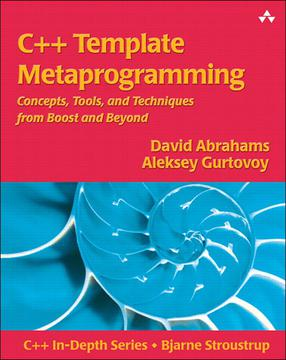
\includegraphics[width=\textwidth]{images/boost_mpl.jpeg}
      \end{column}
      \begin{column}{.2\textwidth}
        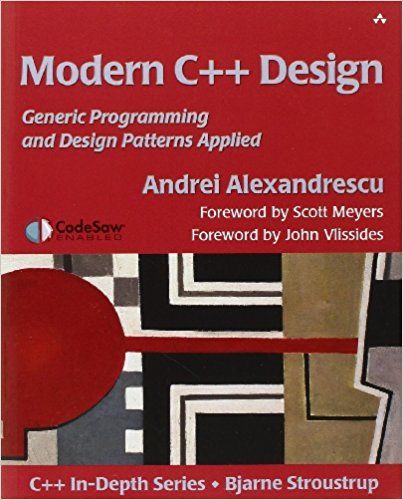
\includegraphics[width=\textwidth]{images/Modern_C++_Design.jpg}
      \end{column}
      \begin{column}{.2\textwidth}
      \end{column}
    \end{columns}
  \item Let's see two use cases
    \begin{itemize}
    \item Type introspection
    \item Computation
    \end{itemize}
  \end{itemize}

\end{frame}

\begin{frame}[fragile]{Type introspection}

  Query the type system to get information about types:
  \begin{itemize}
  \item how big is this type? {\small\code{sizeof(T)}}
  \item is this type default constructible? {\small\code{is\_default\_constructible\_v<T>}}
  \item is this type move-assignable? {\small\code{is\_move\_assignable\_v<T>}}
  \item can the move assignment throw? {\small\code{is\_nothrow\_move\_assignable\_v<T>}}
  \item are these two types the same? \small{\code{is\_same\_v<T1, T2>}}
  \item what's the common type for these types? {\small\code{common\_type\_t<int, unsigned, float>}}
  \end{itemize}

  \begin{codeblock}<2->{
template<typename T>
class uniform_real_distribution \{
  static_assert(std::is_floating_point_v<T>);
  \ddd
\};}\end{codeblock}

\end{frame}

\begin{frame}[fragile]{Iterator traits}

  \code{std::iterator\_traits} is a class template that provides
    properties about an iterator in terms of member types
    \begin{itemize}
    \item \code{\alert<3>{difference\_type}} is a signed integer to identify the
      distance between iterators
    \item \code{value\_type} is the type obtained dereferencing an iterator
    \item \code{pointer} is the type of pointer to \code{value\_type}
    \item \code{reference} is the type of reference to \code{value\_type}
    \item \code{\alert<3>{iterator\_category}} is one of input, output, forward,
      bidirectional, random-access
  \end{itemize}
  
  \begin{codeblock}<2->{
template<typename T>
struct iterator\_traits<T*> // specialization for a pointer
\{
  typedef random_access_iterator_tag iterator_category;
  typedef T                          value_type;
  typedef ptrdiff_t                  difference_type;
  typedef T*                         pointer;
  typedef T&                         reference;
\};}\end{codeblock}
\end{frame}

\begin{frame}[fragile]{Tag dispatching}
  \begin{codeblock}
\uncover<3->{template<class It>
\alt<8->{\alert<8>{auto}}{typename \alert<2>{iterator_traits<It>::difference_type}}
__distance(It first, It last\only<6->{, \alert<6-7>{random_access_iterator_tag} tag}) \{\only<3-5>{ // \alert<3>{for random-access iterators}}
  return last - first;
\}}

\uncover<4->{template<class It>
\alt<8->{\alert<8>{auto}}{typename \alert<2>{iterator_traits<It>::difference_type}}
__distance(It first, It last\only<6->{, \alert<6-7>{input_iterator_tag} tag}) \{\only<4-5>{ // \alert<4>{for input iterators}}
  typename iterator_traits<It>::difference_type n = 0;
  while (first != last) \{ ++first; ++n; \}
  return n;
\}}

template<class It>
\alt<8->{\alert<8>{auto}}{typename \alert<2>{iterator_traits<It>::difference_type}}
\alert<1>{distance}(It first, It last) \{
  \uncover<5->{return __distance(first, last\only<6->{, \alert<6>{iterator_traits<It>::category}\alert<7>{\{\}}});}\only<5>{ // which one?}
\}\end{codeblock}

\end{frame}

\begin{frame}[fragile]{Compile-time computation}

  \begin{itemize}
  \item
    Compute values to be used in contexts where a constant expression is required:
    \begin{itemize}
    \item boolean condition in a \code{static\_assert}
    \item size of an \code{std::array}
    \item \ldots
    \end{itemize}
  \item Statically initialize constant objects
  \item Reduce as much as possible the computation needed at runtime
  \item \ldots
  \end{itemize}

  \uncover<2->{Let's compute the factorial of a number at compile time}
\end{frame}

\begin{frame}[fragile]{Factorial with templates}

  Using a class template and non-type template parameters

  \begin{codeblock}
template<int N>
struct F        \uncover<3->{// general (recursive) case}
\{
  static const int value = \uncover<2->{N * F<N-1>::value};
\};

\uncover<3->{template<>
struct F<0>     // base case
\{
  static const int value = 1;
\};}

static_assert(F<5>::value == 120);
\uncover<4->{std::array<char, F<5>::value> buffer;}\end{codeblock}
\end{frame}

\begin{frame}[fragile]{Factorial with a function}

  Iterative function

  \begin{codeblock}
int factorial(int N) \{
  int r = 1;
  while (N > 0) \{ r *= N-{}-; \}
  return r;
\}\end{codeblock}

Recursive function

\begin{codeblock}
int factorial(int N) \{
  return N == 0 ? 1 : N * factorial(N-1);
\}\end{codeblock}

\begin{codeblock}<2->{
static_assert(\alert<2>{factorial(5)} == 120);    // error
std::array<char, \alert<2>{factorial(5)}> buffer; // error}\end{codeblock}

\end{frame}
\begin{frame}[fragile]{\texttt{constexpr}}

  \begin{itemize}[<+->]
  \item The \code{constexpr} specifier specifies that the value of a variable or
    function can appear in a constant expression
  \item The variable or the function can be evaluated at compile-time
  \item A function can be evaluated at compile-time only if the arguments are
    known at compile-time
    \begin{itemize}
    \item plus a few other constraints
    \end{itemize}
  \end{itemize}

  \begin{codeblock}<+->{
\alert{constexpr} int factorial(int N) \{ // iterative
  int r = 1;
  while (N > 0) \{ r *= N-{}-; \}
  return r;
\}

\alert{constexpr} int factorial(int N) \{ // recursive
  return N == 0 ? 1 : N * factorial(N-1);
\}

\uncover<3->{static_assert(factorial(5) == 120);}
\uncover<4->{\alert{constexpr} auto f5 = factorial(5);
std::array<char, f5> buffer;}}\end{codeblock}
\end{frame}

\begin{frame}[fragile]{\code{if constexpr}}

  Factorial using a function template with a \textit{constexpr-if}

  \begin{codeblock}<2->{
template<int N>
\alert<2>{constexpr} auto Factorial()
\{
  if constexpr (N > 0) \{
    return N * Factorial<N-1>();
  \} else \{
    return 1;
  \}
\}

\uncover<3->{static_assert(\alert<3>{Factorial<5>()} == 120);
constexpr auto f5 = \alert<3>{Factorial<5>()};
std::array<char, f5> buffer;}}\end{codeblock}
  
\end{frame}

\begin{frame}{Hands-on}
  \begin{itemize}
  \item Take the \code{pi} function in \code{pi\_time.cpp} and make it \code{constexpr}
  \item Implement a \code{constexpr} function that checks if a number is prime
  \item Take \code{containers\_assoc.cpp} and extend it to cover also the use of
    the \code{std::set} and \code{std::unordered\_set} associative containers.
    To fill the associative containers you can simply insert all the numbers
    from $0$ to $N$, without random generation and without advancing. In order
    to dispatch to the correct implementation you can use the
    \code{is\_associative} trait already included in that file, using it either
    as a tag or in a \textit{constexpr-if}.
  \item Construct a compile-time table corresponding to a
    \href{https://en.wikipedia.org/wiki/Pascal\%27s_triangle}{Pascal's Triangle}
    of N rows, where N is a compile-time constant.
  \end{itemize}
\end{frame}
